\chapter{Camera calibration}

\begin{description}
    \item[World reference frame (WRF)] \marginnote{World reference frame (WRF)}
        Coordinate system $(X_W, Y_W, Z_W)$ of the real world relative to a reference point (e.g. a corner).

    \item[Camera reference frame (CRF)] \marginnote{Camera reference frame (CRF)}
        Coordinate system $(X_C, Y_C, Z_C)$ that characterizes a camera.

    \item[Image reference frame (IRF)] \marginnote{Image reference frame}
        Coordinate system $(U, V)$ of the image.
        They are obtained as a perspective projection of CRF coordinates as:
        \[ 
            u = \frac{f}{z}x_C 
            \hspace{3em} 
            v = \frac{f}{z}y_C 
        \]

    \begin{figure}[H]
        \centering
        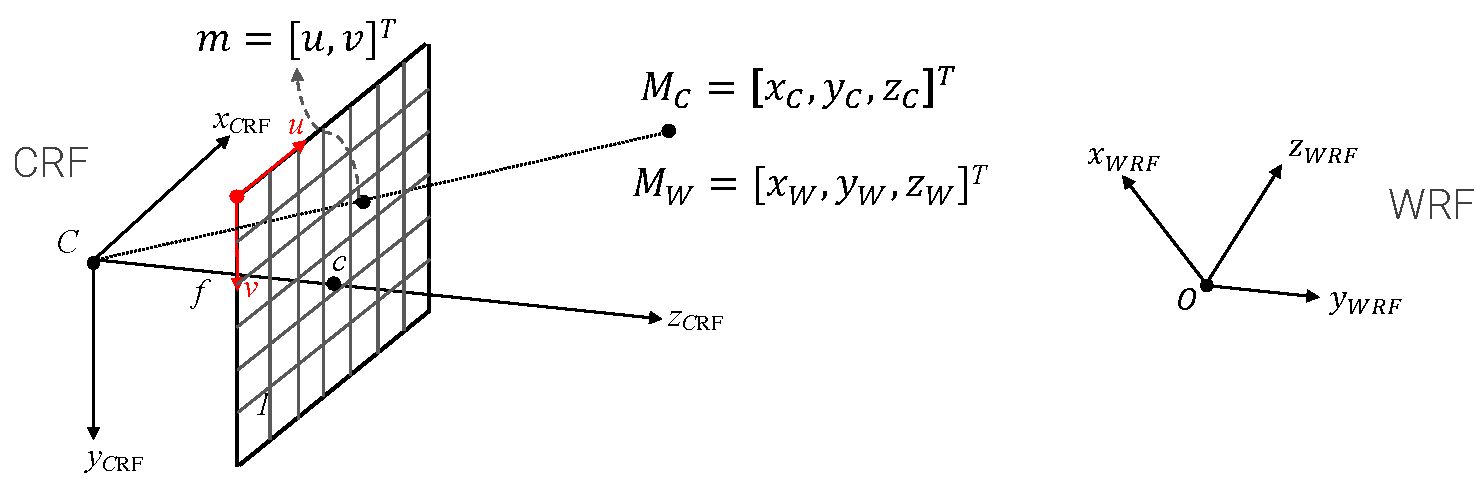
\includegraphics[width=0.8\linewidth]{./img/_formation_system.pdf}
        \caption{Example of WRF, CRF and IRF}
    \end{figure}
\end{description}



\section{Forward imaging model}


\subsection{Image pixelization (CRF to IRF)}
\marginnote{Image pixelization}

The conversion from the camera reference frame to the image reference frame
is done in two steps:
\begin{descriptionlist}
    \item[Discetization] \marginnote{Discetization}
        Given the sizes (in mm) $\Delta u$ and $\Delta v$ of the pixels,
        it is sufficient to modify the perspective projection to map CRF coordinates into a discrete grid:
        \[ 
            u = \frac{1}{\Delta u}\frac{f}{z_C}x_C 
            \hspace{3em} 
            v = \frac{1}{\Delta v}\frac{f}{z_C}y_C 
        \]

    \item[Origin translation] \marginnote{Origin translation}
        To avoid negative pixels, the origin of the image has to be translated from the piercing point $c$ to the top-left corner.
        This is done by adding an offset $(u_0, v_0)$ to the projection (in the new system, $c = (u_0, v_0)$):
        \[ 
            u = \frac{1}{\Delta u}\frac{f}{z_C}x_C + u_0
            \hspace{3em} 
            v = \frac{1}{\Delta v}\frac{f}{z_C}y_C +v_0
        \]

    \begin{figure}[H]
        \centering
        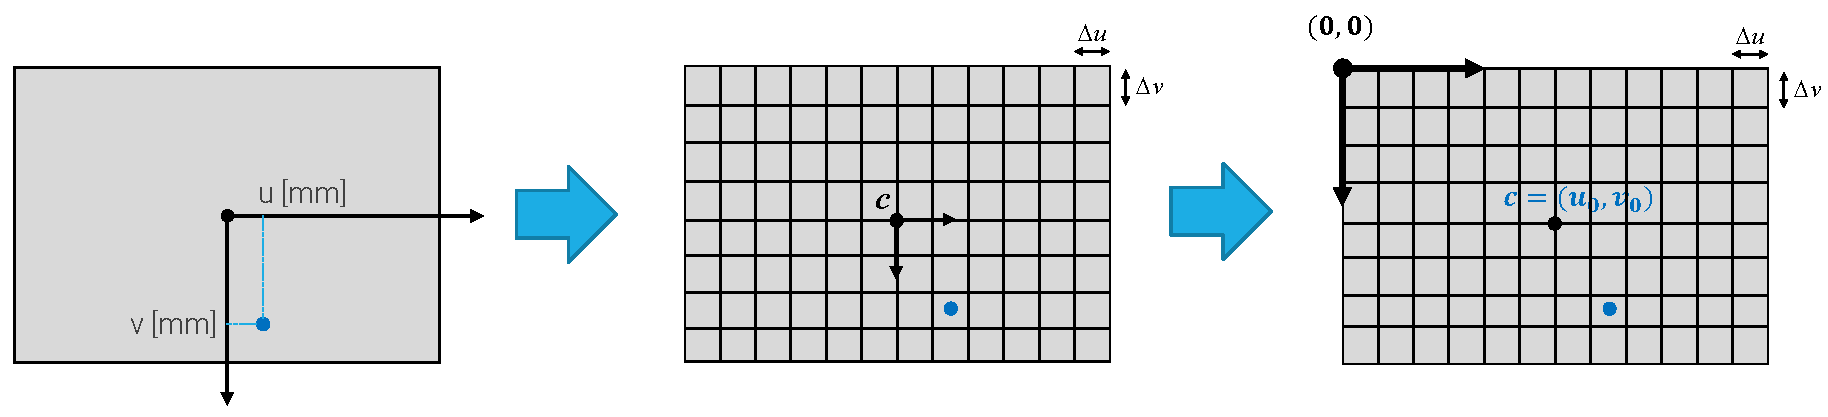
\includegraphics[width=0.9\linewidth]{./img/_pixelization.pdf}
        \caption{Pixelization process}
    \end{figure}

    \item[Intrinsic parameters] \marginnote{Intrinsic parameters}
        By fixing $f_u = \frac{f}{\Delta u}$ and $f_v = \frac{f}{\Delta v}$, the projection can be rewritten as:
        \[ 
            u = f_u\frac{x_C}{z_C} + u_0
            \hspace{3em} 
            v = f_v\frac{y_C}{z_C} +v_0
        \]
        Therefore, there is a total of 4 parameters: $f_u$, $f_v$, $u_0$ and $v_0$.
        
        \begin{remark}
            A more general model includes a further parameter (skew)
            to account for non-orthogonality between the axes of the image sensor such as:
            \begin{itemize}
                \item Misplacement of the sensor so that it is not perpendicular to the optical axis.
                \item Manufacturing issues.
            \end{itemize}

            Nevertheless, in practice skew is always 0.
        \end{remark}
\end{descriptionlist}


\subsection{Roto-translation (WRF to CRF)}
\marginnote{Roto-translation}

The conversion from the world reference system to the camera reference system
is done through a roto-translation wrt the optical center.

Given: 
\begin{itemize}
    \item A WRF point $\vec{M}_W = (x_W, y_W, z_W)$,
    \item A rotation matrix $\matr{R}$,
    \item A translation vector $\vec{t}$,
\end{itemize}
the coordinates $\vec{M}_C$ in CRF corresponding to $\vec{M}_W$ are given by:
\[  
    \vec{M}_C = \begin{bmatrix} x_C \\ y_C \\ z_C \end{bmatrix} =
    \matr{R}\vec{M}_W + \vec{t} =
    \begin{bmatrix}
        r_{1,1} & r_{1,2} & r_{1,3} \\
        r_{2,1} & r_{2,2} & r_{2,3} \\
        r_{3,1} & r_{3,2} & r_{3,3} \\
    \end{bmatrix}
    \begin{bmatrix}
        x_W \\ y_W \\ z_W
    \end{bmatrix}
    +
    \begin{bmatrix}
        t_1 \\ t_2 \\ t_3
    \end{bmatrix}
\]

\begin{remark}
    The coordinates $\vec{C}_W$ of the optical center $\vec{C}$ are obtained as:
    \[ 
        \nullvec = \matr{R}\vec{C}_W + \vec{t} 
            \iff (\nullvec - \vec{t}) = \matr{R}\vec{C}_W 
            \iff \vec{C}_W = \matr{R}^T (\nullvec - \vec{t})
            \iff \vec{C}_W = -\matr{R}^T\vec{t}
    \]
\end{remark}

\begin{description}
    \item[Extrinsic parameters] \marginnote{Extrinsic parameters}
        \phantom{}
        \begin{itemize}
            \item The rotation matrix $\matr{R}$ has 9 elements of which 3 are independent (i.e. the rotation angles around the axes). 
            \item The translation matrix $\vec{t}$ has 3 elements.
        \end{itemize}

        Therefore, there is a total of 6 parameters.
\end{description}


\begin{remark}
    It is not possible to combine the intrinsic camera model and the extrinsic roto-translation to
    create a linear model for the forward imaging model.
    \[
        u = f_u \frac{r_{1,1}x_W + r_{1,2}y_W + r_{1,3}z_W + t_1}{r_{3,1}x_W + r_{3,2}y_W + r_{3,3}z_W + t_3} + u_0
        \hspace{1.5em}
        v = f_v \frac{r_{2,1}x_W + r_{2,2}y_W + r_{2,3}z_W + t_2}{r_{3,1}x_W + r_{3,2}y_W + r_{3,3}z_W + t_3} + v_0
    \]
\end{remark}



\section{Projective space}

\begin{remark}
    In the 2D Euclidean plane $\mathbb{R}^2$, parallel lines never intersect and points at infinity cannot be represented.
    \begin{figure}[H]
        \centering
        \begin{subfigure}{0.45\linewidth}
            \centering
            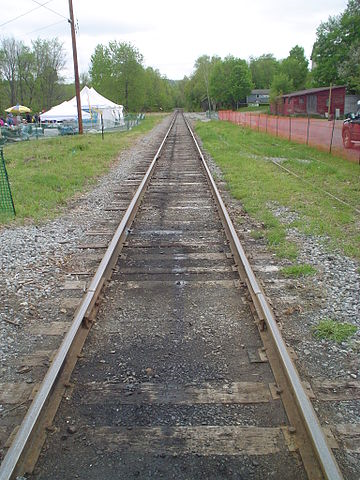
\includegraphics[width=0.45\linewidth]{./img/point_infinity_example1.png}
        \end{subfigure}
        \begin{subfigure}{0.45\linewidth}
            \centering
            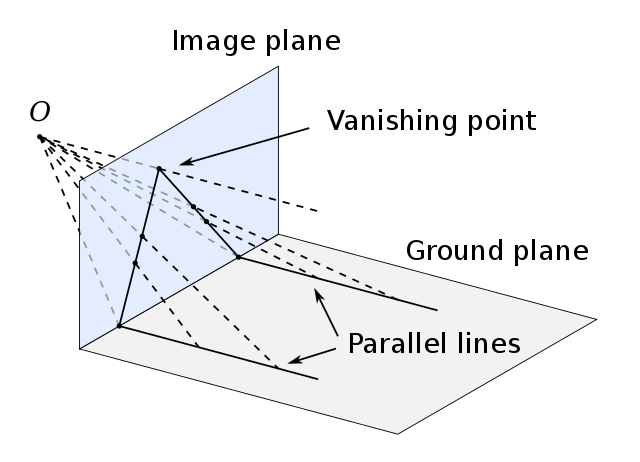
\includegraphics[width=0.8\linewidth]{./img/point_infinity_example2.png}
        \end{subfigure}
        \caption{Example of point at infinity}
    \end{figure}
\end{remark}

\begin{remark}
    Point at infinity is a point in space while the vanishing point is in the image plane.
\end{remark}

\begin{description}
    \item[Homogeneous coordinates] \marginnote{Homogeneous coordinates}
        Without loss of generality, consider the 2D Euclidean space $\mathbb{R}^2$.

        Given a coordinate $(u, v)$ in Euclidean space, its homogeneous coordinates have an additional dimension
        such that:
        \[ (u, v) \equiv (ku, kv, k) \,\forall k \neq 0 \]
        In other words, a 2D Euclidean point is represented by an equivalence class of 3D points.

    \item[Projective space] \marginnote{Projective space}
        Space $\mathbb{P}^n$ associated with the homogeneous coordinates of an Euclidean space $\mathbb{R}^n$.

        \begin{figure}[H]
            \centering
            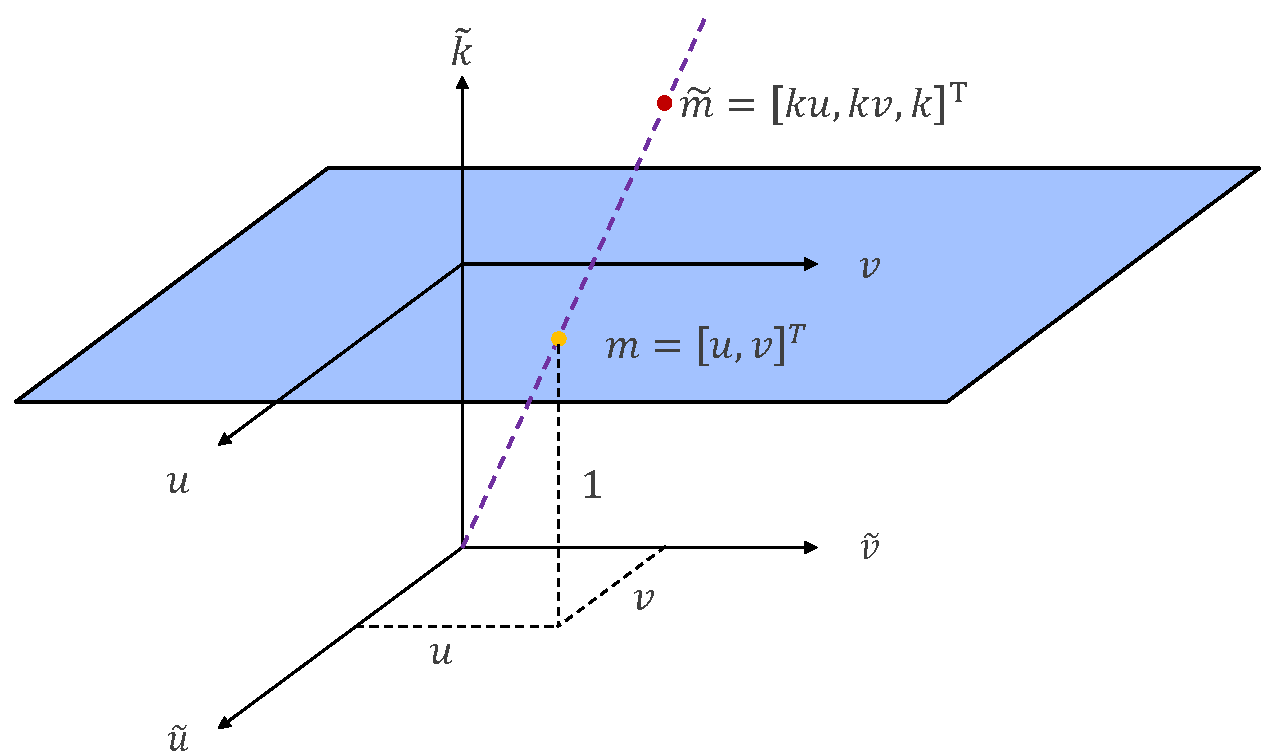
\includegraphics[width=0.6\linewidth]{./img/_projective_space.pdf}
            \caption{Example of projective space $\mathbb{P}^2$}
        \end{figure}

        \begin{remark}
            $\nullvec$ is not a valid point in $\mathbb{P}^n$.
        \end{remark}

        \begin{remark}
            A projective space allows to homogeneously handle both ordinary (image) and ideal (scene) points without introducing additional complexity.
        \end{remark}

    \item[Point at infinity] \marginnote{Point at infinity}
        Given the parametric equation of a 2D line defined as:
        \[ 
            \vec{m} = \vec{m}_0 + \lambda \vec{d} = 
            \begin{bmatrix} u_0 \\ v_0 \end{bmatrix} + \lambda \begin{bmatrix} a \\ b \end{bmatrix} =
            \begin{bmatrix} u_0 + \lambda a \\ v_0 + \lambda b \end{bmatrix}
        \]
        It is possible to define a generic point in the projective space along the line $m$ as:
        \[ 
            \tilde{\vec{m}} \equiv 
            \begin{bmatrix} \vec{m} \\ 1 \end{bmatrix} \equiv
            \begin{bmatrix} u_0 + \lambda a \\ v_0 + \lambda b \\ 1 \end{bmatrix} \equiv
            \begin{bmatrix} \frac{u_0}{\lambda} + a \\ \frac{v_0}{\lambda} + b \\ \frac{1}{\lambda} \end{bmatrix}
        \]

        The projective coordinates $\tilde{\vec{m}}_\infty$ of the point at infinity of a line $m$ is given by:
        \[ \tilde{\vec{m}}_\infty = \lim_{\lambda \rightarrow \infty} \tilde{\vec{m}} \equiv \begin{bmatrix} a \\ b \\ 0 \end{bmatrix} \]

        \begin{figure}[H]
            \centering
            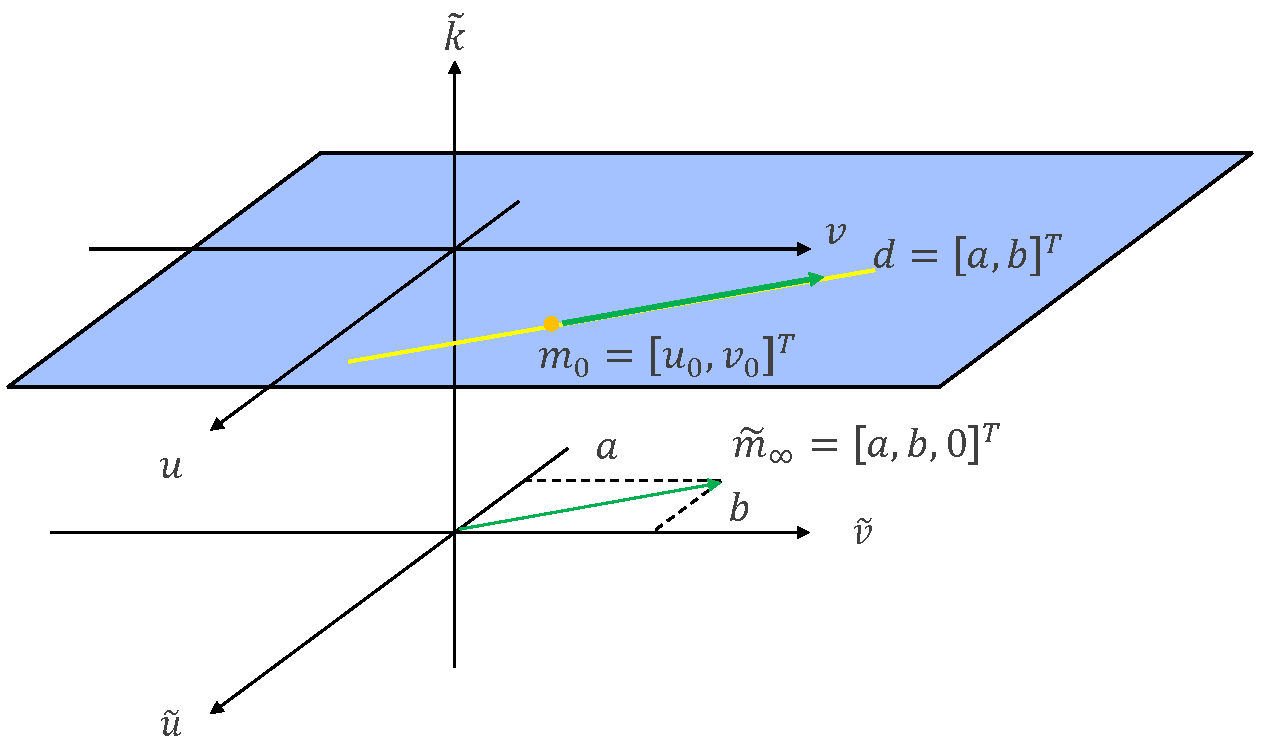
\includegraphics[width=0.6\linewidth]{./img/_projective_point_inifinity.pdf}
            \caption{Example of infinity point in $\mathbb{P}^2$}
        \end{figure}

        In 3D, the definition is trivially extended as:
        \[ 
            \tilde{\vec{M}}_\infty = 
            \lim_{\lambda \rightarrow \infty} \begin{bmatrix} \frac{x_0}{\lambda} + a \\ \frac{y_0}{\lambda} + b \\ \frac{z_0}{\lambda} + c \\ \frac{1}{\lambda} \end{bmatrix} \equiv
            \begin{bmatrix} a \\ b \\ c \\ 0 \end{bmatrix}
        \]

    \item[Perspective projection] \marginnote{Perspective projection in projective space}
        Given a point $\vec{M}_C = (x_C, y_C, z_C)$ in the CRF and its corresponding point $\vec{m} = (u, v)$ in the image,
        the non-linear perspective projection in Euclidean space can be done linearly in the projective space as:
        \[  
            \begin{split}
                \tilde{\vec{m}} &\equiv 
                \begin{bmatrix} u \\ v \\ 1 \end{bmatrix} \equiv
                \begin{bmatrix} f_u\frac{x_C}{z_C} + u_0 \\ f_v\frac{y_C}{z_C} +v_0 \\ 1 \end{bmatrix} \equiv
                z_C \begin{bmatrix} f_u\frac{x_C}{z_C} + u_0 \\ f_v\frac{y_C}{z_C} +v_0 \\ 1 \end{bmatrix} \\
                &\equiv \begin{bmatrix} f_u x_C + z_C u_0 \\ f_v y_C + z_C v_0 \\ z_C \end{bmatrix} \equiv
                \begin{bmatrix} f_u & 0 & u_0 & 0 \\ 0 & f_v & v_0 & 0 \\ 0 & 0 & 1 & 0 \end{bmatrix} \begin{bmatrix} x_C \\ y_C \\ z_C \\ 1 \end{bmatrix} \equiv
                \matr{P}_\text{int} \tilde{\vec{M}}_C
            \end{split}
        \]

        \begin{remark}
            The equation can be written to take account of the arbitrary scale factor $k$ as:
            \[ k\tilde{\vec{m}} = \matr{P}_\text{int} \tilde{\vec{M}}_C \]
            or, if $k$ is omitted, as:
            \[ \tilde{\vec{m}} \approx \matr{P}_\text{int} \tilde{\vec{M}}_C \]
        \end{remark}

        \begin{remark}
            In projective space, we can also project in Euclidean space the point at infinity of parallel 3D lines in CRF with direction $(a, b, c)$:
            \[ 
                \tilde{\vec{m}}_\infty \equiv 
                    \matr{P}_\text{int} \begin{bmatrix} a \\ b \\ c \\ 0 \end{bmatrix} \equiv
                    \begin{bmatrix} f_u & 0 & u_0 & 0 \\ 0 & f_v & v_0 & 0 \\ 0 & 0 & 1 & 0 \end{bmatrix} \begin{bmatrix} a \\ b \\ c \\ 0 \end{bmatrix} \equiv
                    \begin{bmatrix} f_u a + c u_0 \\ f_v b + c v_0 \\ c \end{bmatrix} \equiv
                    c\begin{bmatrix} f_u \frac{a}{c} + u_0 \\ f_v \frac{b}{c} + v_0 \\ 1 \end{bmatrix}
            \]
            Therefore, the Euclidean coordinates are:
            \[ \vec{m}_\infty = \begin{bmatrix} f_u \frac{a}{c} + u_0 \\ f_v \frac{b}{c} + v_0 \end{bmatrix} \]
            
            Note that this is not possible when $c = 0$ (i.e. the line is parallel to the image plane).
        \end{remark}

    \item[Intrinsic parameter matrix] \marginnote{Intrinsic parameter matrix}
        The intrinsic transformation can be expressed through a matrix:
        \[ 
            \matr{A} = 
                \begin{bmatrix}
                    f_u & 0 & u_0 \\ 0 & f_v & v_0 \\ 0 & 0 & 1
                \end{bmatrix} 
        \]
        $\matr{A}$ is always upper right triangular and models the characteristics of the imaging device.
        
        \begin{remark}
            If skew is considered, it would be at position $(1, 2)$.
        \end{remark}

    \item[Extrinsic parameter matrix] \marginnote{Extrinsic parameter matrix}
        The extrinsic transformation can be expressed through a matrix:
        \[ 
            \matr{G} =  
            \begin{bmatrix} \matr{R} & \vec{t} \\ \nullvec & 1 \end{bmatrix} =
            \begin{bmatrix} 
                r_{1,1} & r_{1,2} & r_{1,3} & t_1 \\ 
                r_{2,1} & r_{2,2} & r_{2,3} & t_2 \\ 
                r_{3,1} & r_{3,2} & r_{3,3} & t_3 \\ 
                0 & 0 & 0 & 1
            \end{bmatrix}
        \]

    \item[Perspective projection matrix (PPM)] \marginnote{Perspective projection matrix}
        As the following hold: 
        \[
            \matr{P}_\text{int} = [ \matr{A} | \nullvec ] \hspace{3em} \tilde{\vec{M}}_C \equiv \matr{G} \tilde{\vec{M}}_W
        \]
        The perspective projection can be represented in matrix form as:
        \[ \tilde{\vec{m}} \equiv \matr{P}_\text{int} \tilde{\vec{M}}_C \equiv \matr{P}_\text{int} \matr{G} \tilde{\vec{M}}_W \equiv \matr{P} \tilde{\vec{M}}_W \]
        where $\matr{P} = \matr{P}_\text{int} \matr{G}$ is the perspective projection matrix. It is full-rank and has shape $3 \times 4$.

        \begin{remark}
            Every full-rank $3 \times 4$ matrix is a PPM.
        \end{remark}

        \begin{description}
            \item[Canonical perspective projection] \marginnote{Canonical perspective projection}
                PPM of form:
                \[ \matr{P} \equiv [\matr{I} | \nullvec] \]

                It is useful to represent the core operations carried out by a perspective projection as any general PPM can be factorized as:
                \[ \matr{P} \equiv \matr{A} [\matr{I} | \nullvec] \matr{G} \]
                where:
                \begin{itemize}
                    \item $\matr{G}$ converts from WRT to CRF.
                    \item $[\matr{I} | \nullvec]$ performs the canonical perspective projection (i.e. divide by the third coordinate).
                    \item $\matr{A}$ applies camera specific transformations.
                \end{itemize}

                A further factorization is:
                \[ 
                    \matr{P} \equiv \matr{A} [\matr{I} | \nullvec] \matr{G} \equiv 
                    \matr{A}[\matr{I} | \nullvec] \begin{bmatrix} \matr{R} & \vec{t} \\ \nullvec & 1 \end{bmatrix} \equiv
                    \matr{A} [ \matr{R} | \vec{t} ]
                \]
        \end{description}
\end{description}



\section{Lens distortion}

The PPM is based on the pinhole model and is unable to capture distortions that a lens introduces.

\begin{description}
    \item[Radial distortion] \marginnote{Radial distortion}
        Deviation from the ideal pinhole caused by the lens curvature.

        \begin{descriptionlist}
            \item[Barrel distortion] \marginnote{Barrel distortion}
                Defect associated with wide-angle lenses that causes straight lines to bend outwards.
            \item[Pincushion distortion] \marginnote{Pincushion distortion}
                Defect associated with telephoto lenses that causes straight lines to bend inwards.
        \end{descriptionlist}

        \begin{figure}[H]
            \centering
            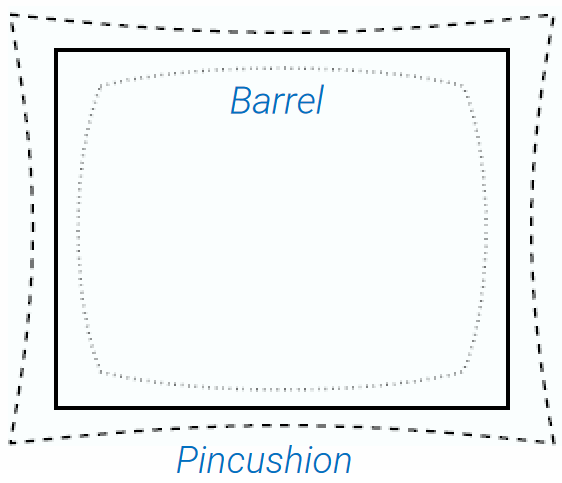
\includegraphics[width=0.25\linewidth]{./img/radial_distortion.png}
            \caption{Example of distortions w.r.t. a perfect rectangle}
        \end{figure}

    \item[Tangental distortion]
        Second-order effects caused by misalignment or defects of the lens (i.e. capture distortions that are not considered in radial distortion).
\end{description}


\subsection{Modeling lens distortion}
\marginnote{Modeling lens distortion}

Lens distortion can be modeled using a non-linear transformation that maps ideal (undistorted) image coordinates $(x_\text{undist}, y_\text{undist})$ into
the observed (distorted) coordinates $(x, y)$:
\[ 
    \begin{bmatrix} x \\ y \end{bmatrix} =
    \underbrace{ L(r) \begin{bmatrix} x_\text{undist} \\ y_\text{undist} \end{bmatrix} }_{\text{Radial distortion}} +
    \underbrace{ \begin{bmatrix} dx(x_\text{undist}, y_\text{undist}, r) \\ dy(x_\text{undist}, y_\text{undist}, r) \end{bmatrix} }_{\text{Tangential distortion}}
\]
where:
\begin{itemize}
    \item $r$ is the distance from the distortion center which is usually assumed to be the piercing point $c = (0, 0)$.
        Therefore, $r = \sqrt{ (x_\text{undist})^2 + (y_\text{undist})^2 }$.
    \item $L(r)$ is the radial distortion function which is a linear operator defined for positive $r$ only and is approximated using the Taylor series:
        \[ L(0) = 1 \hspace{2em} L(r) = 1 + k_1 r^2 + k_2 r^4 + k_3 r^6 + \dots \]
        where $k_i$ are additional intrinsic parameters.
    \item The tangential distortion is approximated as:
        \[ 
            \begin{bmatrix} dx(x_\text{undist}, y_\text{undist}, r) \\ dy(x_\text{undist}, y_\text{undist}, r) \end{bmatrix} =
            \begin{bmatrix} 
                2 p_1 x_\text{undist} y_\text{undist} + p_2 (r^2 + 2(x_\text{undist})^2) \\
                2 p_1 y_\text{undist} x_\text{undist} + p_2 (r^2 + 2(y_\text{undist})^2) \\
            \end{bmatrix}
        \]
        where $p_1$ and $p_2$ are additional intrinsic parameters.
        \begin{remark}
            This approximation has empirically been shown to work.
        \end{remark}
\end{itemize}

\begin{remark}
    The additivity of the two distortions in an assumption.
    Other models might add arbitrary complexity.
\end{remark}


\subsection{Image formation with lens distortion}
\marginnote{Image formation with lens distortion}

Lens distortion is applied after the canonical perspective projection.
Therefore, the complete workflow for image formation becomes the following:
\begin{enumerate}
    \item Transform points from WRF to CRF:
        \[ \matr{G} \tilde{\vec{M}}_W \equiv \begin{bmatrix} x_C & y_C & z_C & 1 \end{bmatrix}^T \]
    \item Apply the canonical perspective projection:
        \[ 
            \begin{bmatrix} \frac{x_C}{z_C} & \frac{y_C}{z_C} \end{bmatrix}^T =
            \begin{bmatrix} x_\text{undist} & y_\text{undist} \end{bmatrix}^T
        \]
    \item Apply the lens distortion non-linear mapping:
        \[ 
            L(r) \begin{bmatrix} x_\text{undist} \\ y_\text{undist} \end{bmatrix} +
            \begin{bmatrix} dx(x_\text{undist}, y_\text{undist}, r) \\ dy(x_\text{undist}, y_\text{undist}, r) \end{bmatrix} =
            \begin{bmatrix} x \\ y \end{bmatrix}
        \]
    \item Transform points from CRF to IRF:
        \[
            \matr{A} \begin{bmatrix} x \\ y \\ 1 \end{bmatrix} \equiv
            \begin{bmatrix} ku \\ kv \\ k \end{bmatrix} \mapsto
            \begin{bmatrix} u \\ v \end{bmatrix}
        \]
\end{enumerate}



\section{Zhang's method}

\begin{description}
    \item[Calibration patterns] \marginnote{Calibration patterns}
        There are two approaches to camera calibration:
        \begin{itemize}
            \item Use a single image of a 3D calibration object (i.e. image with at least 2 planes with a known pattern).
            \item Use multiple (at least 3) images of the same planar pattern (e.g. a chessboard).
        \end{itemize}

        \begin{remark}
            In practice, it is easier to get multiple images of the same pattern.
        \end{remark}
\end{description}

\begin{description}
    \item[Zhang's method] \marginnote{Zhang's method}
        Algorithm to determine the intrinsic and extrinsic parameters of a camera setup given multiple images of a pattern.

        \begin{description}
            \item[Image acquisition] 
                Acquire $n$ images of a planar pattern with $c$ internal corners.

                Consider a chessboard for which we have prior knowledge of:
                \begin{itemize}
                    \item The number of internal corners,
                    \item The size of the squares.
                \end{itemize}

                \begin{remark}
                    To avoid ambiguity, the number of internal corners should be odd along one axis and even along the other
                    (otherwise, a $180^\circ$ rotation of the board would be indistinguishable).
                \end{remark}

                The WRF can be defined such that:
                \begin{itemize}
                    \item The origin is always at the same corner of the chessboard.
                    \item The $z$-axis is at the same level of the pattern so that $z=0$ when referring to points of the chessboard.
                    \item The $x$ and $y$ axes are aligned to the grid of the chessboard. $x$ is aligned along the short axis and $y$ to the long axis.
                \end{itemize}

                \begin{remark}
                    As each image has its own extrinsic parameters,
                    during the execution of the algorithm, for each image $i$ will be computed
                    an estimate of its own extrinsic parameters $\matr{R}_i$ and $\vec{t}_i$.
                \end{remark}

                \begin{figure}[H]
                    \centering
                    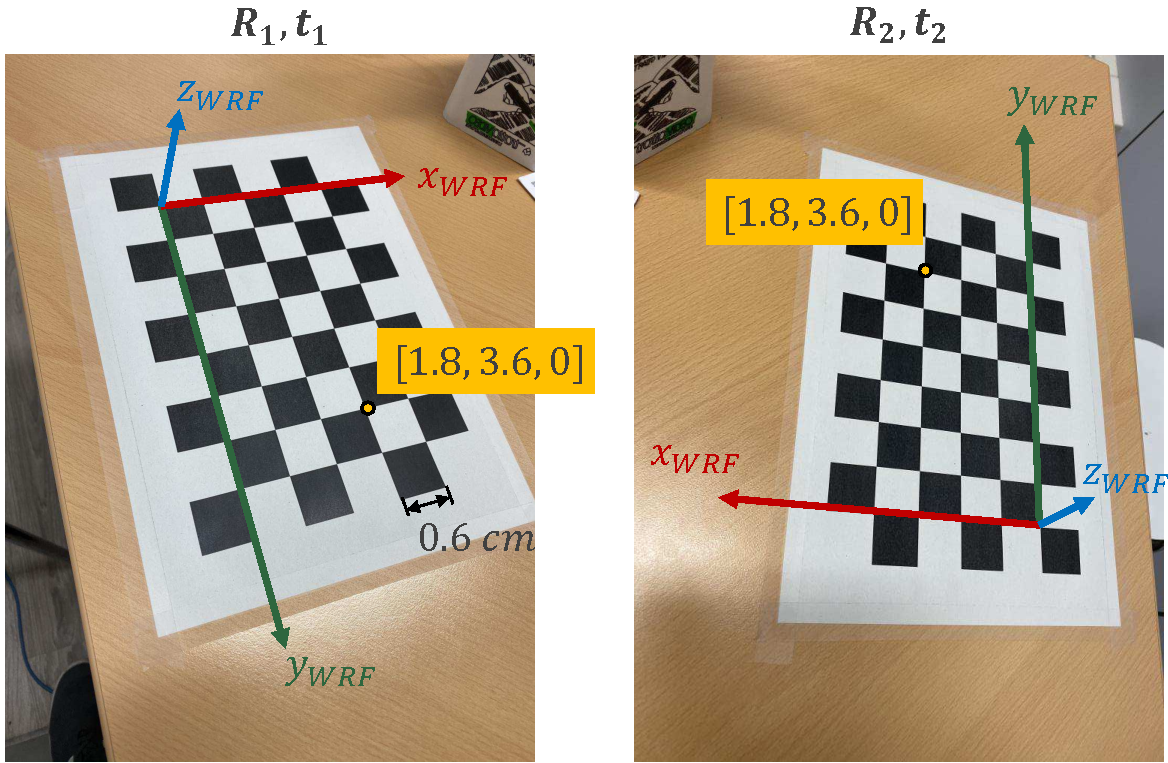
\includegraphics[width=0.45\linewidth]{./img/_zhang_image_acquistion.pdf}
                    \caption{Example of two acquired images}
                \end{figure}
        \end{description}

    \item[Initial homographies guess]
        For each image $i$, compute an initial guess of its homography $H_i$.

        Due to the choice of the $z$-axis position, the perspective projection matrix and the WRF points can be simplified:
        \[ 
            \begin{split}
                k \tilde{\vec{m}} &\equiv 
                k \begin{bmatrix} u \\ v \\ 1 \end{bmatrix} \equiv
                \matr{P} \tilde{\vec{M}}_W \equiv
                \begin{bmatrix}
                    p_{1,1} & p_{1,2} & \cancel{p_{1,3}} & p_{1,4} \\
                    p_{2,1} & p_{2,2} & \cancel{p_{2,3}} & p_{2,4} \\
                    p_{3,1} & p_{3,2} & \cancel{p_{3,3}} & p_{3,4}
                \end{bmatrix}
                \begin{bmatrix} x \\ y \\ \cancel{0} \\ 1 \end{bmatrix} \\
                &\equiv \begin{bmatrix}
                    p_{1,1} & p_{1,2} & p_{1,4} \\
                    p_{2,1} & p_{2,2} & p_{2,4} \\
                    p_{3,1} & p_{3,2} & p_{3,4}
                \end{bmatrix}
                \begin{bmatrix} x \\ y \\ 1 \end{bmatrix} \equiv
                \matr{H}\tilde{\vec{w}}
            \end{split}
        \]
        where $\matr{H}$ is a homography and represents a general transformation between projective planes.

        \begin{description}
            \item[DLT algorithm]
                Consider the $i$-th image with its $c$ corners.
                For each corner $j$, we have prior knowledge of:
                \begin{itemize}
                    \item Its 3D coordinates in the WRF.
                    \item Its 2D coordinates in the IRF.
                \end{itemize}
                Then, for each corner $j$, we can define 3 linear equations where the homography $\matr{H}_i$ of the $i$-th image is the unknown:
                \[ 
                    \tilde{\vec{m}}_{i,j} \equiv 
                        \begin{bmatrix} u_{i,j} \\ v_{i,j} \\ 1 \end{bmatrix} \equiv
                        \begin{bmatrix}
                            p_{i,1,1} & p_{i,1,2} & p_{i,1,4} \\
                            p_{i,2,1} & p_{i,2,2} & p_{i,2,4} \\
                            p_{i,3,1} & p_{i,3,2} & p_{i,3,4} \\
                        \end{bmatrix}
                        \begin{bmatrix} x_j \\ y_j \\ 1 \end{bmatrix} \equiv
                        \matr{H}_i \tilde{\vec{w}}_j \equiv
                        \underset{\mathbb{R}^{3 \times 3}}{\begin{bmatrix}
                            \vec{h}_{i, 1}^T \\ \vec{h}_{i, 2}^T \\ \vec{h}_{i, 3}^T
                        \end{bmatrix}}
                        \tilde{\vec{w}}_j \equiv
                        \underset{\mathbb{R}^{3 \times 1}}{\begin{bmatrix}
                            \vec{h}_{i, 1}^T \tilde{\vec{w}}_j \\ 
                            \vec{h}_{i, 2}^T \tilde{\vec{w}}_j \\ 
                            \vec{h}_{i, 3}^T \tilde{\vec{w}}_j
                        \end{bmatrix}}
                \]
                Geometrically, we can interpret $\matr{H}_i \tilde{\vec{w}}_j$ as a point in $\mathbb{P}^2$
                that we want to align to the projection of $(u_{i,j}, v_{i,j})$ by tweaking $\matr{H}_i$
                (i.e. find $\matr{H}_i^*$ such that $\matr{H}_i^* \tilde{\vec{w}}_j \equiv k \begin{bmatrix} u_{i,j} & v_{i,j} & 1 \end{bmatrix}^T$).
                \begin{center}
                    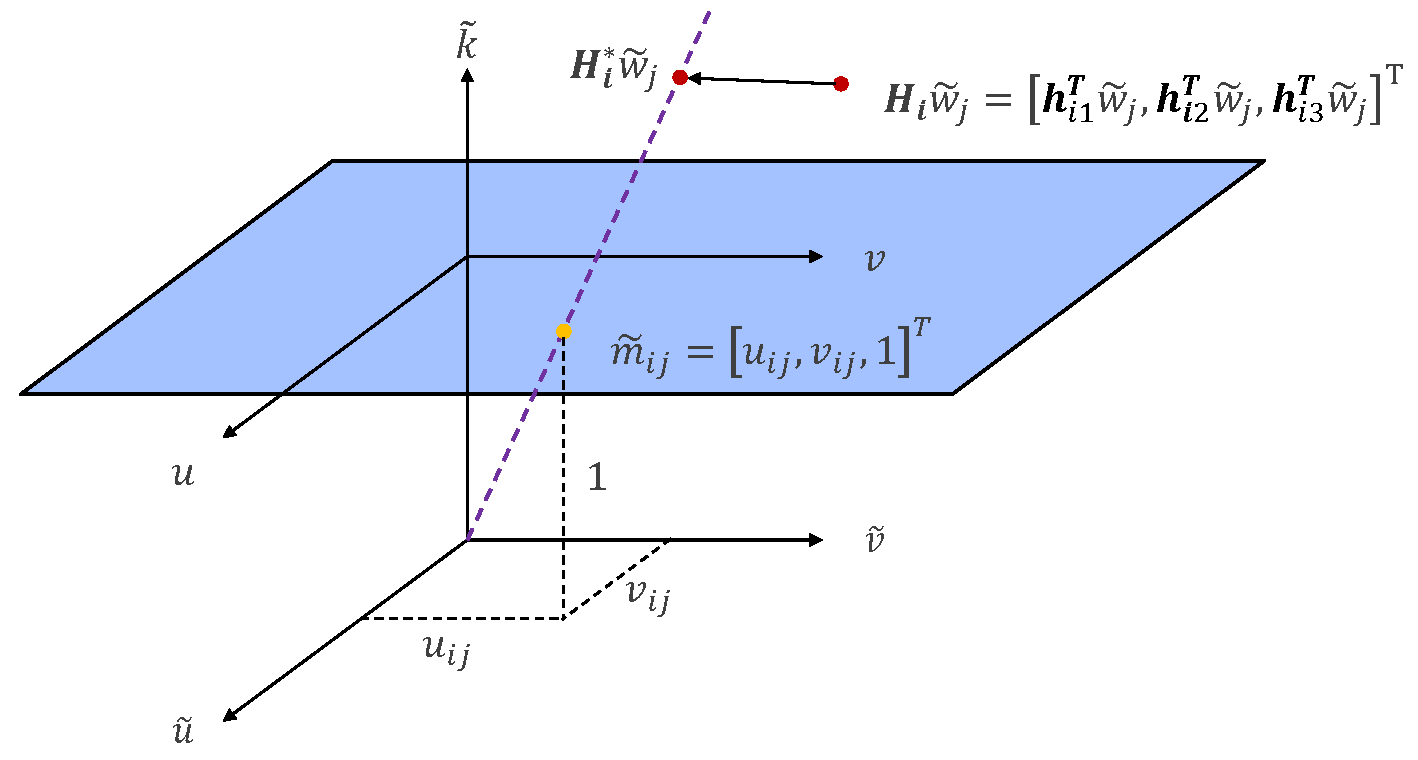
\includegraphics[width=0.7\linewidth]{./img/_zhang_corner_homography.pdf}
                \end{center}

                It can be shown that two points lay on the same line if their cross product is $\nullvec$:
                \begin{align*}
                    \tilde{\vec{m}}_{i,j} \equiv \matr{H}_i \tilde{\vec{w}}_j 
                    &\iff
                        \tilde{\vec{m}}_{i,j} \times \matr{H}_i \tilde{\vec{w}}_j = \nullvec \iff
                        \begin{bmatrix} u_{i, j} \\ v_{i, j} \\ 1 \end{bmatrix} \times
                        \begin{bmatrix}
                            \vec{h}_{i, 1}^T \tilde{\vec{w}}_j \\ 
                            \vec{h}_{i, 2}^T \tilde{\vec{w}}_j \\ 
                            \vec{h}_{i, 3}^T \tilde{\vec{w}}_j
                        \end{bmatrix} =
                        \begin{bmatrix} 0 \\ 0 \\ 0 \end{bmatrix} 
                    \\
                    &\iff
                        \begin{bmatrix}
                            v_{i,j} \vec{h}_{i,3}^T \tilde{\vec{w}}_j - \vec{h}_{i, 2}^T \tilde{\vec{w}}_j \\
                            \vec{h}_{i, 1}^T \tilde{\vec{w}}_j - u_{i, j} \vec{h}_{i, 3}^T \tilde{\vec{w}}_j \\
                            u_{i, j} \vec{h}_{i, 2}^T \tilde{\vec{w}}_j - v_{i, j} \vec{h}_{i, 1}^T \tilde{\vec{w}}_j
                        \end{bmatrix} =
                        \begin{bmatrix} 0 \\ 0 \\ 0 \end{bmatrix} 
                    \\
                    &\iff
                        \underset{\mathbb{R}^{3 \times 9}}{\begin{bmatrix}
                            \nullvec_{1\times 3} & -\vec{w}_j^T & v_{i,j}\vec{w}_j^T \\
                            \vec{w}_j^T & \nullvec_{1\times 3} & -u_{i,j} \vec{w}_j^T \\
                            -v_{i,j} \vec{w}_j^T & u_{i,j} \vec{w}_j^T & \nullvec_{1\times 3}
                        \end{bmatrix}}
                        \underset{\mathbb{R}^{9 \times 1}}{\begin{bmatrix}
                            \vec{h}_{i,1} \\ \vec{h}_{i,2} \\ \vec{h}_{i,3}
                        \end{bmatrix}}
                        =
                        \begin{bmatrix} 0 \\ 0 \\ 0 \end{bmatrix} 
                    & \text{\parbox[t]{5cm}{$\vec{h}_{*}^T \tilde{\vec{w}}_j = \tilde{\vec{w}}_j^T \vec{h}_{*}$\\and factorization}} \\
                    &\iff
                        \underset{\mathbb{R}^{2 \times 9}}{\begin{bmatrix}
                            \nullvec_{1\times 3} & -\vec{w}_j^T & v_{i,j}\vec{w}_j^T \\
                            \vec{w}_j^T & \nullvec_{1\times 3} & -u_{i,j} \vec{w}_j^T \\
                        \end{bmatrix}}
                        \underset{\mathbb{R}^{9 \times 1}}{\begin{bmatrix}
                            \vec{h}_{i,1} \\ \vec{h}_{i,2} \\ \vec{h}_{i,3}
                        \end{bmatrix}}
                        =
                        \begin{bmatrix} 0 \\ 0 \end{bmatrix} 
                    & \text{\parbox{5cm}{only the first two\\equations are\\linearly independent}} \\
                \end{align*}
        \end{description}

    \item[Homographies refinement]
    \item[Initial intrinsic parameters guess]
    \item[Initial extrinsic parameters guess]
    \item[Initial distortion parameters guess]
    \item[Parameters refinement]
\end{description}